\chapter{Zweites Kaptitel}
\blindtext
\blinditemize
\section{Erster Abschnitt}
\blindmathpaper

In Abbildung \ref{MeinBild} ist was tolles zu sehen.
\begin{figure}[h]
	\centering
	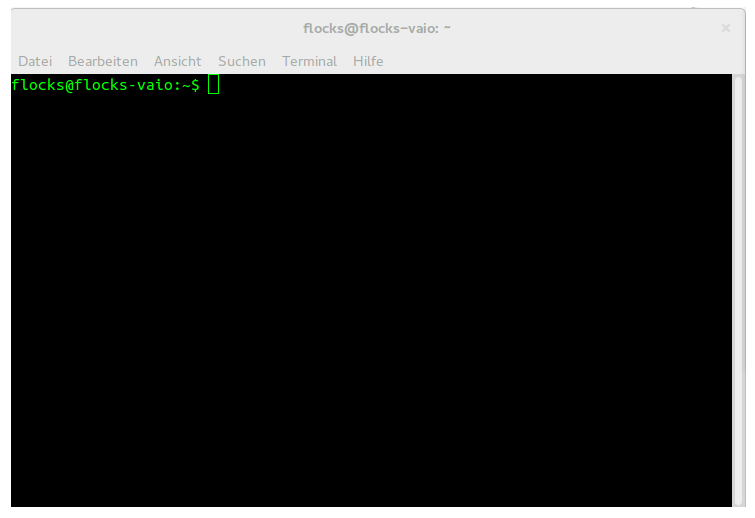
\includegraphics[width=.7\textwidth] {Bilder/bild.png}
	\caption{Screenshot}\label{MeinBild}
\end{figure}
\FloatBarrier
\blindtext
\section{Zweiter Abschnitt}
\setlength\extrarowheight{5pt}
\begin{table}[h]
	\begin{center}
	\begin{tabular}{ l l p{.5\textwidth} }
		\hline
		\emph{Model} & \textbf{RezeptZutaten.java} & Ein Softwaremodell für die Zutaten des anzuzeigenden Rezeptes. Die Datei stellt Methoden und Funktionen bereit, mit der nötige Zutaten für dieses Rezept wiedergegeben werden können. Dies kann von einer beliebigen Quelle sein. Beispielsweise über eine Schnittstelle zu einer Datenbank.\\[.2cm]
		\emph{View} & \textbf{RezeptView.jsp} & Die Werte, die aus dem Model übergeben werden, zeigt die RezeptView.jsp auf der Oberfläche an. Sie ist für das Präsentieren der Daten für den Benutzer zuständig. In diesen Dateien kann Logik enthalten sein, sollte aber nicht.\\[.2cm]
		\emph{Controller} & \textbf{RezeptAction.java} & Diese Datei ist die Verbindung zwischen der View und dem Model. Es wird entschieden, welche Aktion des Nutzers welche Reaktion zur Folge hat und die definierte View ausgewählt. Des Weiteren leitet sie die Daten aus dem Model an diese weiter. \\[.2cm]
		\hline
	\end{tabular}\caption{Beispieltabelle mit Zitat (vgl. \cite[S.~21]{struts})}
\end{center}
\end{table}
\FloatBarrier